%
% File acl2010.tex
%
% Contact  jshin@csie.ncnu.edu.tw or pkoehn@inf.ed.ac.uk
%%
%% Based on the style files for ACL-IJCNLP-2009, which were, in turn,
%% based on the style files for EACL-2009 and IJCNLP-2008...

%% Based on the style files for EACL 2006 by 
%%e.agirre@ehu.es or Sergi.Balari@uab.es
%% and that of ACL 08 by Joakim Nivre and Noah Smith

\documentclass[11pt]{article}
\usepackage{acl2010}
\usepackage{times}
\usepackage{url}
\usepackage{latexsym}
\usepackage{graphicx}
\usepackage{amssymb}
%\setlength\titlebox{6.5cm}    % You can expand the title box if you
% really have to
\usepackage{color}

\definecolor{red}{rgb}{1,0,0}

\newcommand{\mnote}[1]{\marginpar{%
  \vskip-\baselineskip
  \raggedright\footnotesize
  \itshape\hrule\smallskip\tiny{#1}\par\smallskip\hrule}}  

\newcommand{\mtodo}[1]{\mnote{\textcolor{red}{#1}}}

\title{Bilingual Lexicon Induction from Monolingual Sources \\ for Low Resource Languages}

%\author{Blah\\
%  JHU\\
%  Madltimore, MD.\\
%  {\tt blah@jhu.edu}  \And
%  Blah\\
%  JHU\\
%  Baltimore, MD.\\
%  {\tt  blah@jhu.edu}}

\date{}

\begin{document}
\maketitle
\begin{abstract}
Statistical machine translation relies on the
availability of substantial amounts of human translated texts (\emph{bitexts})
for parameter estimation. Such bilingual resources are available for relatively few
language pairs, which presents obstacles to applying current statistical translation models to low-resource languages. In this work, we induce bilingual dictionaries from more plentiful monolingual corpora 
using a diverse set of cues, including: cross-lingual vector space models, the frequencies of words over time, orthographic similarity, etc.  We report the efficacy of these monolingual cues and contrast their performance for a language pair where plentiful bilingual resources are available.  We further evaluate the accuracy of bilingual dictionaries induced between English and XX, YY, ZZ.  Rather than evaluate only on the 1000 most frequent nouns, as previous work on lexicon induction has done, we further evaluate on a random sample of lower frequency words. 
We introduce a novel, space-efficient
extension to the \emph{locality sensitive hashing} (LSH) scheme that exploits cross-lingual, phrasal
distributional statistics.



\end{abstract}

\section{Introduction} \label{sect:intro}


Statistical methods for machine translation continue to push the state of the
art in automatic translation. However, they crucially rely on the availability
of large numbers of translations aligned across two languages. Generation of
these parallel corpora require the efforts of bilingual speakers and are
extremely expensive to produce in sufficient quantities to induce a high quality
statistical translation system. As a result, these methods can not be
successfully applied to the majority of word's languages and especially those
less frequently taught. In terms of the community's evaluation of progress, most
shared tasks involve european languages for which generous quantities of
multilingual parliament proceedings are available.

At the same time we now have unprecedented access to vast and continually
expanding monolingual resources. Moreover, they often contain additional
metadata which can provide non-sentential cues for inducing bilingual resources;
suggesting we might substantially reduce and eventually eliminate the
requirement for explicitly aligned bilingual translations. Recent examples
include exploiting temporal information to induce Named Entity lexicons
(\cite{Alex, David}), and topic information to generate translations
(\cite{Mimno}). Moreover, resources such as these are likely to be extremely
useful for numerous multilingual NLP tasks (\mtodo{Examples}).

\section{Inducing Bilingual Lexicons} \label{sect:lexinduct}

Our goal is to generate bilingual resources for pairs of languages for which we
have sufficient monolingual data. These languages currently include \mtodo{List
  languages}.

This article consitutes the first report on this effort: since more data is
continuously becoming available, we expect to add more languages to this list in
the future. 
%We propose to induce \emph{comprehensive} bilingual token and
%multi-token (phrasal) lexicons for each of those languages and English.

Cues and similarity metrics:
\begin{itemize}
\setlength{\parskip}{0pt}
  \item Context (including contextual NEs), using dependency contexts for the resources rich side (i.e. English).
  \item Time
  \item Topics (i.e. wiki categories)
  \item Edit distance
\end{itemize}

\noindent Combination strategies:
\begin{itemize}
\setlength{\parskip}{0pt}
  \item cue scores as classification features: use seed dictionaries for supervised data.
  \item rank aggregation
\end{itemize}


\section{Contextual Similarity}

Grouping semantically related words through distributional statistics (e.g.
\cite{Pereira:1993}) is a way to reduce both the search space and associate
translations. We can find associations between clusters instead of individual
lexemes or phrases, by intersecting them we can substantially reduce the space
of possible translations (Fig. \ref{fig:semclusters}). \mtodo{Verbiage is very
  close to CCB's proposal}.

\begin{figure}
\centerline{\mbox{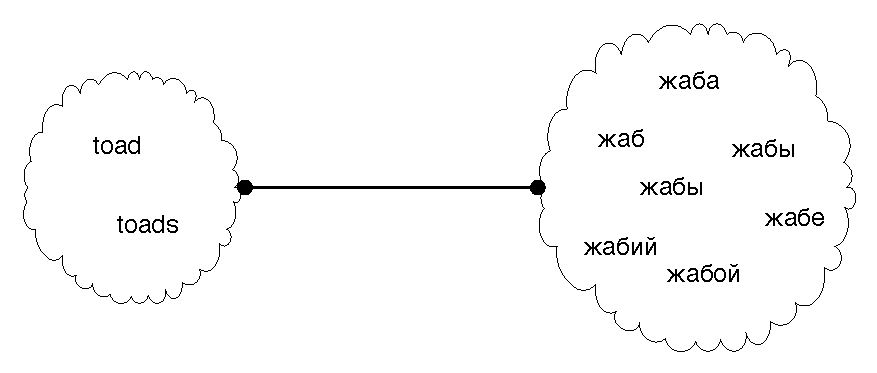
\includegraphics[width=3.5in]{figures/morphology}}}
\caption{Inducing lexicons using contextual similarity.  An example set of word forms for \emph{toad} for English and Russian.}
\label{fig:cycle} \label{fig:morphology}
\end{figure}

%% {\bf Unsupervised Morphology Induction.} Many of the languages in our list such
%% as Russian, Arabic, Korean (\todo{Make sure they end up in our list}) have rich
%% morphology (Figure \ref{fig:morphology}). These languages are characterized by
%% morphological rules generating a large number of word forms for the same lexeme
%% (\todo{Reasonable enough?} and present a substantial challenge for our setting,
%% since we cannot assume that such linguistic knowledge is available for our
%% languages of interest. We will exploit alternative unsupervised (such as
%% \cite{Goldwater}) or weakly supervised techniques to group word forms in order
%% to collect accurate corpus statistics needed for our methods.

\begin{figure}
\centerline{\mbox{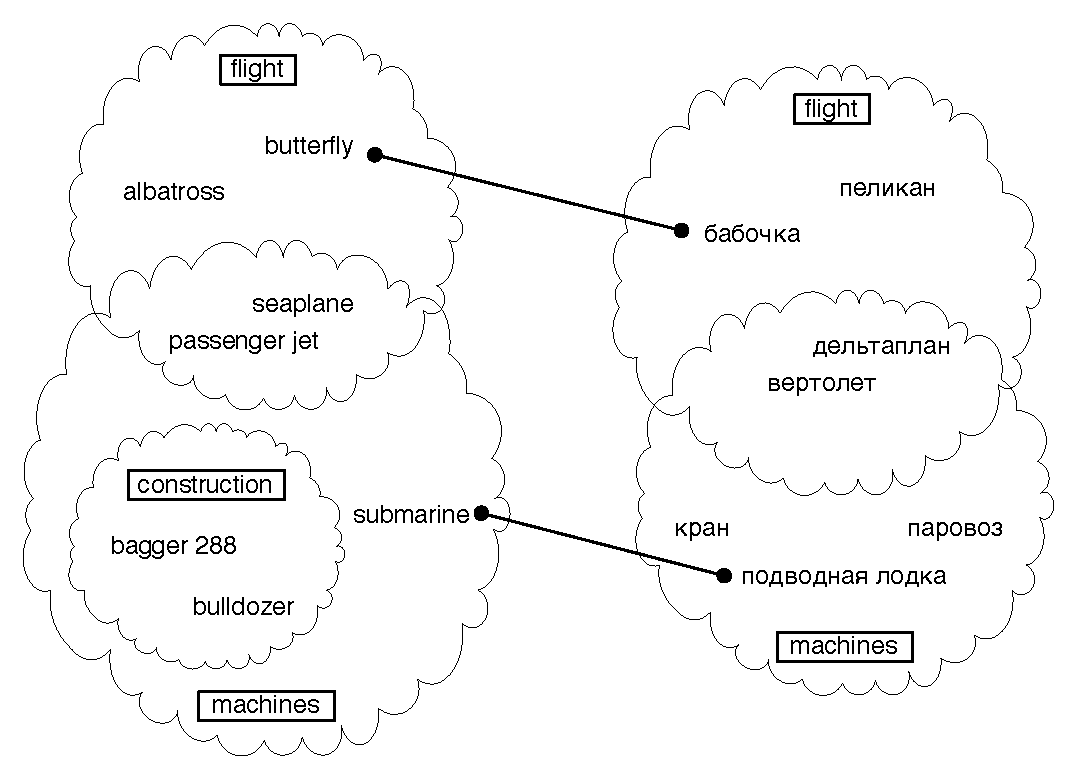
\includegraphics[width=3.5in]{figures/semclusters}}}
\caption{Hierarchical clustering:  associations can be inferred between sets of semantically related words.  Intersections between sets e.g. ``flying machines'') can also substantially limit the sets of potential translation candidates. }
\label{fig:cycle} \label{fig:semclusters}
\end{figure}


\begin{figure}
\centerline{\mbox{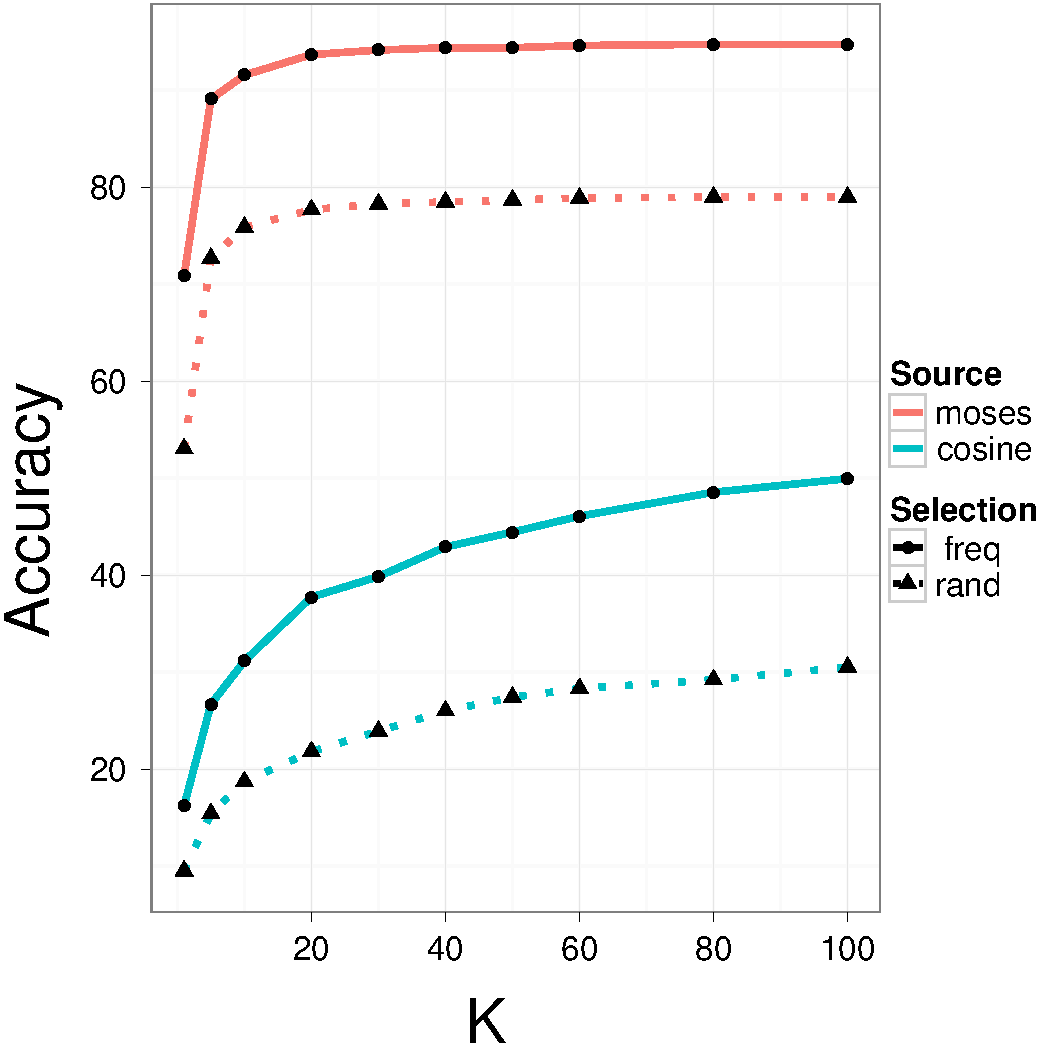
\includegraphics[width=2.8in]{figures/Moses-v-Cosine}}}
\caption{Moses as compared to cosine.}
\label{fig:moses-v-cosine}
\end{figure}





\section{Experimental Evaluation} \label{sect:exp}
\noindent Evaluation:  tokens for inducing translations.  Evaluation metrics: why precision at top-k?

\subsection{Data and Other Resources}

Describe the data:
\begin{itemize}
  \item Wiki
  \item News
\end{itemize}

\noindent Describe the resources:
\begin{itemize}
  \item Dictionaries: generally, noisy
  \item Parallel data: some languages may have small amounts of parallel data
\end{itemize}

\subsection{Quality of Available Resources}

Parallel data experiments:
\begin{itemize}
  \item Moses lexical tables vs. monolingual cues (e.g., Fig. \ref{fig:parvsmono}).
  \item Use Moses lexical tables as seed dictionaries.
\end{itemize}

\begin{figure}
\begin{center}
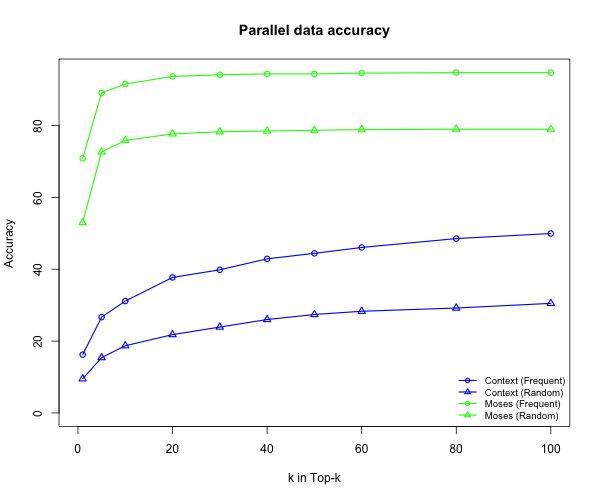
\includegraphics[width=3in]{figures/mostfreqrand.png}
\caption{Bilingual lexicons from Moses lexical tables vs. using contextual cues.} \label{fig:parvsmono}
\end{center}
\end{figure}

\subsection{Quality of Individual Cues} 

Performance of individual cues per language.

\subsection{Combination strategies}

Classification and rank aggregation.

%% vandurme> put here as placeholder, feel free to move about paper as needed
\include{lsh}

\section{Related Work} \label{sect:relwork}

\begin{itemize}
\setlength{\parskip}{0pt}
  \item Context: \cite{Rapp:1995,Rapp:1999,Fung:1998}
  \item Time: \cite{Schafer:2002,Klementiev:2006b}
  \item Topics: \cite{Mimno:2009,Boyd-Graber:2009}
  \item Multiple: \cite{Schafer:2002,Koehn:2000,Haghighi:2008}
  \item Dependecies: \cite{Garera:2009}
  \item Bridge languages: \cite{Mann:2001}
  \item Combination Strategies: \cite{Koehn:2000,Klementiev:2006b,Klementiev:2008a}
  \item Mechanical Turk: Our NAACL workshop paper.
  \item Other: \cite{Monz:2005}
\end{itemize}

\section{Conclusions and Future Work} \label{sect:conclusions}

Using cues for MT.

%% \section*{Acknowledgments}

\bibliographystyle{acl}
\bibliography{references}

\end{document}
